\documentclass[a4paper,12pt,twoside]{memoir}

% Castellano
\usepackage[spanish,es-tabla]{babel}
\selectlanguage{spanish}
\usepackage[utf8]{inputenc}
\usepackage[T1]{fontenc}
\usepackage{lmodern} % Scalable font
\usepackage{microtype}
\usepackage{placeins}

\RequirePackage{booktabs}
\RequirePackage[table]{xcolor}
\RequirePackage{xtab}
\RequirePackage{multirow}

% Links
\usepackage[colorlinks]{hyperref}
\hypersetup{
	allcolors = {red}
}

% Ecuaciones
\usepackage{amsmath}

% Rutas de fichero / paquete
\newcommand{\ruta}[1]{{\sffamily #1}}

% Párrafos
\nonzeroparskip


% Imagenes
\usepackage{graphicx}
\newcommand{\imagen}[2]{
	\begin{figure}[!h]
		\centering
		\includegraphics[width=0.9\textwidth]{#1}
		\caption{#2}\label{fig:#1}
	\end{figure}
	\FloatBarrier
}

\newcommand{\imagenflotante}[2]{
	\begin{figure}%[!h]
		\centering
		\includegraphics[width=0.9\textwidth]{#1}
		\caption{#2}\label{fig:#1}
	\end{figure}
}



% El comando \figura nos permite insertar figuras comodamente, y utilizando
% siempre el mismo formato. Los parametros son:
% 1 -> Porcentaje del ancho de página que ocupará la figura (de 0 a 1)
% 2 --> Fichero de la imagen
% 3 --> Texto a pie de imagen
% 4 --> Etiqueta (label) para referencias
% 5 --> Opciones que queramos pasarle al \includegraphics
% 6 --> Opciones de posicionamiento a pasarle a \begin{figure}
\newcommand{\figuraConPosicion}[6]{%
  \setlength{\anchoFloat}{#1\textwidth}%
  \addtolength{\anchoFloat}{-4\fboxsep}%
  \setlength{\anchoFigura}{\anchoFloat}%
  \begin{figure}[#6]
    \begin{center}%
      \Ovalbox{%
        \begin{minipage}{\anchoFloat}%
          \begin{center}%
            \includegraphics[width=\anchoFigura,#5]{#2}%
            \caption{#3}%
            \label{#4}%
          \end{center}%
        \end{minipage}
      }%
    \end{center}%
  \end{figure}%
}

%
% Comando para incluir imágenes en formato apaisado (sin marco).
\newcommand{\figuraApaisadaSinMarco}[5]{%
  \begin{figure}%
    \begin{center}%
    \includegraphics[angle=90,height=#1\textheight,#5]{#2}%
    \caption{#3}%
    \label{#4}%
    \end{center}%
  \end{figure}%
}
% Para las tablas
\newcommand{\otoprule}{\midrule [\heavyrulewidth]}
%
% Nuevo comando para tablas pequeñas (menos de una página).
\newcommand{\tablaSmall}[5]{%
 \begin{table}
  \begin{center}
   \rowcolors {2}{gray!35}{}
   \begin{tabular}{#2}
    \toprule
    #4
    \otoprule
    #5
    \bottomrule
   \end{tabular}
   \caption{#1}
   \label{tabla:#3}
  \end{center}
 \end{table}
}

%
% Nuevo comando para tablas pequeñas (menos de una página).
\newcommand{\tablaSmallSinColores}[5]{%
 \begin{table}[H]
  \begin{center}
   \begin{tabular}{#2}
    \toprule
    #4
    \otoprule
    #5
    \bottomrule
   \end{tabular}
   \caption{#1}
   \label{tabla:#3}
  \end{center}
 \end{table}
}

\newcommand{\tablaApaisadaSmall}[5]{%
\begin{landscape}
  \begin{table}
   \begin{center}
    \rowcolors {2}{gray!35}{}
    \begin{tabular}{#2}
     \toprule
     #4
     \otoprule
     #5
     \bottomrule
    \end{tabular}
    \caption{#1}
    \label{tabla:#3}
   \end{center}
  \end{table}
\end{landscape}
}

%
% Nuevo comando para tablas grandes con cabecera y filas alternas coloreadas en gris.
\newcommand{\tabla}[6]{%
  \begin{center}
    \tablefirsthead{
      \toprule
      #5
      \otoprule
    }
    \tablehead{
      \multicolumn{#3}{l}{\small\sl continúa desde la página anterior}\\
      \toprule
      #5
      \otoprule
    }
    \tabletail{
      \hline
      \multicolumn{#3}{r}{\small\sl continúa en la página siguiente}\\
    }
    \tablelasttail{
      \hline
    }
    \bottomcaption{#1}
    \rowcolors {2}{gray!35}{}
    \begin{xtabular}{#2}
      #6
      \bottomrule
    \end{xtabular}
    \label{tabla:#4}
  \end{center}
}

%
% Nuevo comando para tablas grandes con cabecera.
\newcommand{\tablaSinColores}[6]{%
  \begin{center}
    \tablefirsthead{
      \toprule
      #5
      \otoprule
    }
    \tablehead{
      \multicolumn{#3}{l}{\small\sl continúa desde la página anterior}\\
      \toprule
      #5
      \otoprule
    }
    \tabletail{
      \hline
      \multicolumn{#3}{r}{\small\sl continúa en la página siguiente}\\
    }
    \tablelasttail{
      \hline
    }
    \bottomcaption{#1}
    \begin{xtabular}{#2}
      #6
      \bottomrule
    \end{xtabular}
    \label{tabla:#4}
  \end{center}
}

%
% Nuevo comando para tablas grandes sin cabecera.
\newcommand{\tablaSinCabecera}[5]{%
  \begin{center}
    \tablefirsthead{
      \toprule
    }
    \tablehead{
      \multicolumn{#3}{l}{\small\sl continúa desde la página anterior}\\
      \hline
    }
    \tabletail{
      \hline
      \multicolumn{#3}{r}{\small\sl continúa en la página siguiente}\\
    }
    \tablelasttail{
      \hline
    }
    \bottomcaption{#1}
  \begin{xtabular}{#2}
    #5
   \bottomrule
  \end{xtabular}
  \label{tabla:#4}
  \end{center}
}



\definecolor{cgoLight}{HTML}{EEEEEE}
\definecolor{cgoExtralight}{HTML}{FFFFFF}

%
% Nuevo comando para tablas grandes sin cabecera.
\newcommand{\tablaSinCabeceraConBandas}[5]{%
  \begin{center}
    \tablefirsthead{
      \toprule
    }
    \tablehead{
      \multicolumn{#3}{l}{\small\sl continúa desde la página anterior}\\
      \hline
    }
    \tabletail{
      \hline
      \multicolumn{#3}{r}{\small\sl continúa en la página siguiente}\\
    }
    \tablelasttail{
      \hline
    }
    \bottomcaption{#1}
    \rowcolors[]{1}{cgoExtralight}{cgoLight}

  \begin{xtabular}{#2}
    #5
   \bottomrule
  \end{xtabular}
  \label{tabla:#4}
  \end{center}
}


















\graphicspath{ {./img/} }

% Capítulos
\chapterstyle{bianchi}
\newcommand{\capitulo}[2]{
	\setcounter{chapter}{#1}
	\setcounter{section}{0}
	\chapter*{#2}
	\addcontentsline{toc}{chapter}{#2}
	\markboth{#2}{#2}
}

% Apéndices
\renewcommand{\appendixname}{Apéndice}
\renewcommand*\cftappendixname{\appendixname}

\newcommand{\apendice}[1]{
	%\renewcommand{\thechapter}{A}
	\chapter{#1}
}

\renewcommand*\cftappendixname{\appendixname\ }

% Formato de portada
\makeatletter
\usepackage{xcolor}
\newcommand{\tutor}[1]{\def\@tutor{#1}}
\newcommand{\course}[1]{\def\@course{#1}}
\definecolor{cpardoBox}{HTML}{E6E6FF}
\def\maketitle{
  \null
  \thispagestyle{empty}
  % Cabecera ----------------
\noindent
\includegraphics[width=\textwidth]{cabecera}\vspace{1cm}%
  \vfill
  % Título proyecto y escudo informática ----------------
  \colorbox{cpardoBox}{%
    \begin{minipage}{.8\textwidth}
      \vspace{.5cm}\Large
      \begin{center}
      \textbf{TFG del Grado en Ingeniería Informática}\vspace{.6cm}\\
      \textbf{\LARGE\@title{}}
      \end{center}
      \vspace{.2cm}
    \end{minipage}

  }%
  \hfill\begin{minipage}{.20\textwidth}
    
\includegraphics[width=\textwidth]{escudoInfor}
  \end{minipage}
  \vfill
  % Datos de alumno, curso y tutores ------------------
  \begin{center}%
  {%
    \noindent\LARGE
    Presentado por \@author{}\\ 
    en Universidad de Burgos --- \@date{}\\
    Tutor: \@tutor{}\\
  }%
  \end{center}%
  \null
  \cleardoublepage
  }
\makeatother

\newcommand{\nombre}{Jesús Carro Tomé} %%% cambio de comando

% Datos de portada
\title{título del TFG}
\author{\nombre}
\tutor{nombre tutor}
\date{\today}

\begin{document}

\maketitle


\newpage\null\thispagestyle{empty}\newpage


%%%%%%%%%%%%%%%%%%%%%%%%%%%%%%%%%%%%%%%%%%%%%%%%%%%%%%%%%%%%%%%%%%%%%%%%%%%%%%%%%%%%%%%%
\thispagestyle{empty}


\noindent
\includegraphics[width=\textwidth]{cabecera}\vspace{1cm}

\noindent D. nombre tutor, profesor del departamento de nombre departamento, área de nombre área.

\noindent Expone:

\noindent Que el alumno D. \nombre, con DNI 71308125Y, ha realizado el Trabajo final de Grado en Ingeniería Informática titulado título de TFG. 

\noindent Y que dicho trabajo ha sido realizado por el alumno bajo la dirección del que suscribe, en virtud de lo cual se autoriza su presentación y defensa.

\begin{center} %\large
En Burgos, {\large \today}
\end{center}

\vfill\vfill\vfill

% Author and supervisor
\begin{minipage}{0.45\textwidth}
\begin{flushleft} %\large
Vº. Bº. del Tutor:\\[2cm]
D. nombre tutor
\end{flushleft}
\end{minipage}
\hfill
\begin{minipage}{0.45\textwidth}
\begin{flushleft} %\large
%Vº. Bº. del co-tutor:\\[2cm]
%D. nombre co-tutor
\end{flushleft}
\end{minipage}
\hfill

\vfill

% para casos con solo un tutor comentar lo anterior
% y descomentar lo siguiente
Vº. Bº. del Tutor:\\[2cm]
D. nombre tutor


\newpage\null\thispagestyle{empty}\newpage




\frontmatter

% Abstract en castellano
\renewcommand*\abstractname{Resumen}
\begin{abstract}
En este proyecto se llevará acabo una aplicación de escritorio, desarrollada en python, que propone en base a las caracteristicas físicas del usuario, una serie de opciones, enseñandole a comer saludablemente, y mostrandole sus progresos.
\end{abstract}

\renewcommand*\abstractname{Descriptores}
\begin{abstract}
Aplicación de escritorio, dietoterapía, analisis y administración de datos\ldots
\end{abstract}

\clearpage

% Abstract en inglés
\renewcommand*\abstractname{Abstract}
\begin{abstract}
Se aborda la \textbf{dietoterapía} mezclada con las \textbf{nuevas tecnologías} para un sencillo aprendizaje de estas.
\end{abstract}

\renewcommand*\abstractname{Keywords}
\begin{abstract}
dietoterapía, salud, python, analisis de datos, mejor condicion fisica, \ldots
\end{abstract}

\clearpage

% Indices
\tableofcontents

\clearpage

\listoffigures

\clearpage

\listoftables
\clearpage

\mainmatter
\capitulo{1}{Introducción}

Este proyecto, desarrollado en Python, nace de la idea de una aplicación nueva de enseñanza dieto-terapéutica. Este trabajo, en cierto modo, hace honor al propio nombre de " informática ", llevando a los usuarios una información, que como se demuestran en diversos estudios citados y desarrollados mas adelante en esta memoria, la mayoría de gente desconoce; y automatizando de manera ágil y transparente al usuario el aprendizaje exhaustivo sobre la dieto-terapia, para conseguir que el usuario consiga un habito de vida saludable y no reciba una estricta dieta imposible de seguir. \\
Actualmente se estima que alrededor del 81 por ciento de los españoles, que se proponen cambiar de hábitos y seguir una dieta acaba desistiendo. Eso en su mayoría nace de la dificultad, de mantener un ritmo constante de rigor a la hora de seguir una serie de instrucciones que de una manera u otra te condicionan, impidiéndote hacer una vida 100 por ciento, más allá de lo que en el ámbito alimenticio se refiere, como es en el ámbito social. \\
Por ello, Combinando el análisis y tratamiento de datos, mediante sistemas informáticos; con los últimos estudios relacionados con la dieto-terapia. Se busca crear una aplicación, que más que inculcar una dieta al usuario, sirva de guía para percibir un nuevo estilo de vida como propio. Gracias a esto, se puede llegar a conseguir un gran avance medico/informático, debido a la importancia que la dieto-terapia tiene en la salud de las personas. \\
Se calcula que una de cada cinco muertes en el mundo esta relacionada con la mala alimentación, por supuesto, dejando fuera las muertes por desnutrición. Por lo tanto, el proyecto es sustenta, de la constante necesidad y la creciente demanda de sistemas que ayuden y faciliten a una adecuada alimentación o dieto-terapia para el cuidado personal. Se pensó en un modelo de auto-aprendizaje, debido a que se ha considerado que pese a ser más lento es más sencillo para el ser humano adecuar un estilo de vida, que no seguir una dieta estricta. La idea principal es que el usuario, en base a sus necesidades, elija de manera libre el menú que vaya a consumir en cada plato a lo largo del día, teniendo en cuenta en todo momento, como de bueno o mala es esa decisión para él. \\
\begin{quote}
El estilo de aprendizaje auto-aprendizaje es mas efectivo cuando reconoces que es lo mas importante para ti ”
\cite{autoaprendizaje}
\end{quote}
Tras estudiar varios métodos de aprendizaje, se consideró, que debido a la relación directa: dieta/salud, el auto-aprendizaje sería el mas oportuno, de esta manera a un ritmo lento y constante, el usuario aprende a comer bien, y no se pierde entre dietas.
Se pensaron en una serie de pasos imprescindibles para inculcar un nuevo estilo de vida:

\begin{enumerate}
\item	Identificar que se quiere cambiar
\item	Metas específicas, realistas y constantes
\item	Creación de un plan
\item	Recordatorios que seguir
\item	Mide tus avances
\end{enumerate}
Se ha buscado que la herramienta desarrollada durante todos estos meses, de una sensación de falsa simplicidad, es decir, se ha buscado hacer lo mas simple, para abordar cuestiones complejas, de manera común, sin rizar el rizo, pero evitando dejar el mínimo de cabos sueltos, se ha buscado cumplir de manera pasiva cada uno de estos puntos dentro de la aplicación, puesto que dentro de sus objetivos y funcionalidades esta:

\begin{enumerate}
\item	Su función principal, aprender, y cambiar el estilo de vida a través de la dietoterapia, cumpliendo el objetivo uno, de identificar que parte de tu estilo de vida, deseas cambiar.
\item	Posiblemente, una de las partes mas complicadas e invisibles del proyecto. El proyecto siempre va a recomendar lo que considera la mejor opción, y siempre va a ser en base a los datos del cliente, consiguiendo, que las metas sean constantes, y que poco a poco se vayan volviendo mas estrictas, y pase de manera imperceptible al usuario.
\item	Creación de un plan, la mas fácil e importante de los cinco pasos. Si se piensa detenidamente, es el usuario el que se crea su propio plan, pero siempre teniendo una “mano invisible”, que le ayudo a redirigir sus opciones, se decir, cada cosa que decide el usuario dentro de la aplicación queda registrada, y se ve en los gráficos sobre la calidad, como en verdad ha comido nuestro cliente.
\item Igual es la menos intuitiva para el usuario, pero no nos olvidamos de ella, se encuentra en el historial, esos gráficos que permiten ver al usuario como avanza y en la barra que le dice como esta comiendo en el día. Dentro de estas opciones aparecen reflejados los puntos 4 y 5.
\end{enumerate}

A lo largo de esta memoria será plausible el como se ha desarrollado cada parte del proyecto, tanto en el ámbito informático como en el nutricional. Detallando cada estudio, desarrollo y opción que se ha tenido a lo largo de este, para que toda decisión tomada a lo largo del periodo de desarrollo quede clara, y se entienda el ¿por qué?, de cada decisión. Con este proyecto se consigue proyectar la unión de dos mundos complejos, de la manera más simple posible, haciendo alarde de que en la sencillez se oculta la complejidad de todo esto.

\capitulo{2}{Objetivos del proyecto}

Este apartado explica de forma precisa y concisa cuales son los objetivos que se persiguen con la realización del proyecto. Se puede distinguir entre los objetivos marcados por los requisitos del software a construir y los objetivos de carácter técnico que plantea a la hora de llevar a la práctica el proyecto.

\capitulo{3}{Conceptos teóricos}

\section{Introducción}
Se explicará todo concepto teórico interno y/o externo, usados sobre la metodología del programa para su correcto funcionamiento y la coherencia entre funciones, acercándose al máximo a la experiencia real que se quiere conseguir con este proyecto, a la hora de interconectar los datos con los métodos dando el mayor rigor en cuanto a veracidad.
\section{Nutrición}
Es uno de los ámbitos principales de estudio a lo largo de este proyecto, para la máxima veracidad de los resultados. En cada calculo y método que se realizan en el programa, se tienen en cuenta una serie de valores y datos, meticulosamente estudiados para poder usarlos en el programa.\\

La nutrición como avance médico, es un tema que, a día de hoy, esta en pleno auge, numerosos estudios resaltan el estrecho vinculo entre un buen estilo de vida y una buena calidad de vida en cuanto al termino de salud se refiere. Ya no solo en patologías directamente relacionadas con la alimentación, sino en otro tipo de patologías mas graves, las cuales se puede reducir enormemente el riesgo con una buena alimentación.\cite{prevCancer}
\subsection{Reparto calórico}

Aunque durante el periodo de investigación se ha demostrado que todos los nutrientes principales de un alimento son igual de buenos y necesarios, si que es verdad que la predisposición del cuerpo ante la comida varía según la etapa del día. \\

Durante el desayuno somos mas propensos a asimilar los alimentos, mientras que a la hora de la cena nuestro metabolismo está más ralentizado, por lo que hay que cenar con mayor moderación, pero no es aconsejable restringirlo estrictamente.\\

Para ello se realizó un estudio contrastando diferentes datos y se calculó a través de los datos obtenidos el porcentaje total de cada macronutriente en cada comida.
\subsubsection{Reparto total de los macronutrientes}
Hay que tener en cuenta que este proyecto ha sido diseño para personas con diferentes patologías y que como tal, tendrán diferentes distribuciones, en un principio se pensó en todas las combinaciones posibles: baja en grasa, alta en grasa, baja en hidratos, alta en hidratos, etc.\\

Pero tras hablar con una profesional endocrina en el Hospital Universitario de Burgos, María Maravi, me afirmo que: 
\begin{quote}
Nosotros no trabajamos con dietas altas o bajas en hidratos, pues son necesarios por igual para todo el mundo y por lo cual, la modificación de este solo puede traer problemas al paciente. Un diabético ha de tomar la cantidad normal de hidratos
\end{quote}
De este modo la Doctora nos proporcionó una tabla con las diferentes variaciones.
\tablaSmall{Distintos tipos de dietas y su distribución}{l c c c c}{distribucionDietas}
{ \multicolumn{1}{l}{Dietas} & Hidratos & Grasa & Proteínas & Ejemplos\\}{ 
Normal & 55\% & 20\% & 25\% & Cualquier persona  \\
Baja en grasa & 55\% & 15\% & 30\% & Problemas cardiovasculares \\
Baja en proteína & 55\% & 25\% & 20\%  & Problemas de hígado \\
Alta en proteína & 50\% & 15\% & 35\% & Alta actividad física \\
} 
\subsection{Reparto total calórico}
Internamente se realizan múltiples cálculos, los cuales son necesarios ya sea para la correcta recomendación alimenticia del usuario, como para el correcto tratamiento de los datos. \\

Debido a la diversidad de información encontrada en la web, fue muy complicado llegar a un punto estable donde los datos tuvieran una coherencia para todos y fueran veraces. Para que las cifras cuadrase se creo una  matriz donde se dividían las columnas por macronutrientes y las filas por el tipo de comida concreto. Esta matriz debía tener como resultado un porcentaje que cuadrase en varios ejes y un sub-porcentaje que cuadrase en el total, de esta manera se tenía controlado en todo momento la veracidad de los datos.
\tablaSmall{Distintos tipos de dietas y su distribución}{l c c c c}{distribucionDietas}
{ \multicolumn{1}{l}{Comidas} & Grasa & Hidratos & Proteínas & carga TOTAL \\}{ 
Desayuno & 15\% & 30\% & 24\% & 24.75\%  \\
Almuerzo & 10\% & 25\% & 14\% & 13.5\%\\
Comida & 20\% & 25\% & 24\%  & 30.5\% \\
Merienda & 20\% & 10\% & 14\% & 11.5\% \\
Cena & 10\% & 10\% & 24\% & 19.75\% \\
} 
Se estudio para ello la diferente predisposición de las comidas, y los nutrientes internos de cada uno.
\subsection{Nutriscore (Algoritmo del semaforo)}
De manera objetiva, se creó un método de medición para la conveniencia de los alimentos(calidad). para que dicho calculo, mantuviese correlación con la actualidad que cubre el proyecto, se decidió usar el recurso Nutriscore, actualmente usado en España.\\

A continuación, se muestra en imagen el algoritmo seguido de una breve explicación:\\
\imagen{Nutriscore}{Algoritmo Nutriscore}

La imagen anterior muestra el algoritmo , el cual, se basa en el sumatorio de una serie de valores negativos ( Tabla roja), los cuales reciben una puntuación en base a la cantidad de ese nutriente informativo en nuestro alimento. Y una serie de valores positivos (Tabla verde), que funciona de la misma manera que lo anterior. Se hace la diferencia entre ambas puntuaciones y en base al resultado se le asigna un valor de la A a la E, con diferentes colores, que hace visible la calidad del alimento.
\section{Prevenciones}
Debido al propósito del proyecto como ayuda a la prevención o avance de enfermedades/patologías por parte del usuario, había que estudiar que tipo de prevenciones había y donde cabía el proyecto.
Tipos:
\begin{itemize}
\item	Prevención Primaria: Evita la adquisición de la enfermedad. Estas técnicas actúan suprimiendo los factores desfavorables antes de que puedan llegar a general la enfermedad.
\item	Prevención Secundaria: Detectar la enfermedad y evitar su posible progresión. Interviene cuando se inicia la enfermedad, y su función principal es que el diagnostico y tratamiento precoz mejores el pronostico y control de las enfermedades.
\item	Prevención Terciaria: Comprende aquellas medidas dirigidas al tratamiento y a la rehabilitación, además de la ralentización de su progresión. Interviene cuando las lesiones son irreversibles, y la enfermedad está arraigada, pudiendo llegar a ser crónica.
\end{itemize}
\cite{prevencion}

Una vez, pautado los puntos de prevención, ¿Dónde entre la nutrición?\\
La detención primera es clara, una buena alimentación junto con una serie de hábitos de vida saludables puede impedir enormemente el desarrollo de la enfermedad, siendo una de las recomendaciones mas repetidas por los profesionales a sus pacientes.
En la detención secundaría también entra esta categoría, es más complicado encontrar fuentes que lo verifiquen, pero existen cada vez más estudios como los citados en el apartado 6. Un buen habito de vida puede tener hasta mejores resultados que la medicación en algunos casos.
En el caso de la detención terciaria es más complicado de asegurar, con el tiempo se va aceptando en mayor medida que un buen habito de vida puede ayudar a este tipo de prevenciones, y varios profesionales en la materia lo corroboran, pero la realidad es que, a falta de estudios concluyentes a día de hoy, no se puede afirmar con exactitud.\\

Lo que si es cierto es que una buena alimentación, junto con actividad física moderada a lo largo de la vida, siempre es recomendable para la salud de cualquier persona.\\
\section{Enseñanza}
La idea principal del proyecto es evitar otra aplicación repetitiva sobre la gestión o impartición de dietas, las cuales suelen ser abandonadas por la mayoría de los españoles al paso del tiempo.\\

Para ello se estudio varios métodos de enseñanza, aprendizaje a través de métodos multimedia, etc. 
\subsection{Métodos multimedia}
En los últimos años, el desarrollo de aplicaciones tanto móviles como de escrito han sido integradas activamente en los diferentes métodos de enseñanza. Se considera que las aplicaciones a día de hoy ofrecen muchas ventajas al mundo de la enseñanza:
\begin{itemize}
\item	Comunicación a tiempo real entre el método de enseñanza y el alumno estando siempre al alcance de éste
\item	Cómoda distribución de tareas, siendo más fácil el orden y la organización.
\item	Ayuda a la superación de las barreras geográficas.
\end{itemize}

En educación, se a pronosticado a que lo largo de los años dominará el uso de la Tablet. Por ello parte de la progresión del proyecto , es su extensión a Tablets y Smartphones.\cite{enseñanza}
\subsection{Autoaprendizaje}
Debido a que el uso de este tipo de aplicaciones carece de una figura presenta durante la fase de aprendizaje del usuario, se buscó un método en el que el usuario por su propia índole, aprendiese, y poco a poco fuese adecuando su nuevo habito de vida, en base a sus propias elecciones. Esto daba al usuario versatilidad, dándole la opción en todo momento de elegir que es lo que mas le apeteciese, recomendando la mejor opción y complicando que el usuario hago una mala elección, de esta manera se juega con la idea de hacer creer al usuario que es el, el que toma las buenas o malas decisiones.
\section{Autoaprendizaje del programa}
Pese a que en ningún momento se llego a implantar debido a que quedaba fuera del objetivo final. Se desarrollo un estudio sobre inteligencia artificial o redes neuronales en la aplicación para hacer de la aplicación un sistema único, que aprenda del usuario que hace uso de ella, y de esta manera, abandonar la idea actualmente extendida de formulas genéricas, en cuanto a aplicaciones y cálculos del TMB se refiere y ofrecer una experiencia totalmente personalizada.\\

Se realizó un estudio de redes neuronales, llegando a crear una red de tres capas, bastante básica, sin usar ningún de las librerías proporcionada por Python.\\

Se ideo añadir dicha neurona a una función que fuera la auto-selección de los menús, pero esto solo reforzaría las elecciones mas comunes del usuario que no tienen por qué ser las mejores.\\

Tras meditarlo con cautela, se pensó que en caso de tener una base de datos más extensa, su uso, sería el entrenamiento de la red en base al historial de todos los usuarios, y  tras pasar el usuario en forma de vector, ver cual sería de todos, el valor inicial optimo del TMB, (para ser exactos de la suma que se la añade más adelante para mantener, bajar o subir), y además crear una adaptabilidad de esto, haciendo que si la próxima vez que el usuario edite su peso, no ha bajado, subido o mantenido, lo que debería haber hecho, se le sume una cantidad estandarizada, de esta manera, el programa va aprendiendo a base del uso, y con el tiempo daría el resultado mas personal y exacto posible.\\
\section{Métodos de recomendación}
Se meditaron diferentes métodos de recomendación:
\begin{itemize}
\item	Filtro colaborativo Basado en modelos: Utilizan los datos para ajustar modelos que después pueden ser utilizados para proponer recomendaciones.
\item	Filtro colaborativo basado en usuario: Es un tipo de filtro basado en memoria, y se basa en recomendar lo que usuarios similares a nuestro usuario han escogido.
\item	“Vecino mas cercano”: Su calculo se basa en la correlación de Pearson, y es muy similar (por no decir idéntico) al filtro colaborativo basado en usuarios.
\end{itemize}

Todos estos métodos, son métodos ampliamente utilizados por grandes distribuidores como Amazon, Netflix ...\\
Pero para este proyecto presentaban dos grandes inconvenientes:
\begin{itemize}
\item	Como bien se vio en la asignatura de gestión de la información, son métodos que requieren de muchos usuarios y productos para que funcionen de manera precisa, sino las recomendaciones pueden ser totalmente aleatorias, dando paso a una muy mala recomendación.
\item	La mas importante, si este proyecto es creado por el desconocimiento extendido sobre la buena alimentación y sus beneficios no podemos compara un usuario con el resto de usuarios, pues a la larga, el programa se “estropeará”, y pasará a dividir a las personas en dos grandes grupos: Los que se cuidan bien y los que no. Y es precisamente lo que se quiere evitar.
\end{itemize}

Por ello, pese a ser uno de los filtros menos recomendados en la asignatura de Gestión de la información, irónicamente para este proyecto fue el más apropiado. Se paso a usar un filtro basado en contenidos, por lo general, este filtro necesita saber las características del usuario y del contenido de los productos (en este caso alimentos), para poder realizar la recomendación. Esto obviamente tiene por lo general un gran coste de información y por ello no es recomendable. Pero en este proyecto se parte con esa información. Básicamente, sabiendo exactamente las características que el usuario busca en esa comida, se le recomienda dicha el producto (Menú), que mas se adapte a lo que busca.



\capitulo{4}{Técnicas y herramientas}

Apartado cuyo objetivo es presentar las técnicas metodológicas y las herramientas de desarrollo que se han utilizado para llevar a cabo el proyecto. Si se han estudiado diferentes alternativas de metodologías, herramientas, bibliotecas, etcétera.\\

Se comenta los aspectos más destacados de cada opción, con un repaso somero a los fundamentos esenciales y referencias bibliográficas para que el lector pueda ampliar su conocimiento sobre el tema.
\section{¿Por qué Python?}
La razón es la sencillez y capacidad de este lenguaje para el análisis y tratamiento de los datos, gracias a librerías como Pandas o Numpy. Base gran parte de la metodología de análisis usada en este proyecto en el libro: Python for Data Analysis. \cite{analisis}
\\ 
Las distintas posibilidades cotejadas antes de empezar fueron: Java, Android, R y Python. El primero en ser descartado fue Java, tras un estudio inicial sobre como se quería desarrollar la aplicación. Después de buscar entre diferentes fuentes; Java no era la mejor opción, dichas fuentes siempre te orientaban hacia Python y/o R, debido a la cantidad de librerías enfocadas al análisis y tratamiento de los datos que estos poseen.\\
La razón por la que se planteo Android fue por que este trabajo está desarrollado para unir el mundo de la dietoterapia, y las ciencias de la Salud con la informática. La forma más clara y rápida de llevar al usuario dichas tecnologías es a través de un  SmartPhone, pero se acabó descartando debido a la falta de conocimientos sobre sistemas Android. A estas alturas ya solo existían dos opciones:  Python y R.\\
Tras indagar superficialmente sobre ambos lenguajes para el análisis y el tratamiento de datos, se llego a la conclusión que ambos lenguajes tienen una forma de trabajar muy similares,y  debido a que durante los años de estudio el alumno ha trabajado en numerosas ocasiones con Python, se decantó por Python.
\section{Metodología}
\subsection{Introduccón}
En este apartado se explicará el cómo y porque se ha tratado los datos en este trabajo,  además de los diferentes cálculos internos que se realizan para el sistema de recomendaciones, cálculos, etc.
\subsection{Excell y Pandas}
Se ha usado la herramienta de Microsoft Excel, para simular una base de datos, trabajando los datos en formato DataFrame. Los DataFrame son proporcionados por la librería Pandas. Existen diferentes hojas de cálculo, que funcionan como colecciones de una base de datos. Estas hojas son explicadas más adelante.
\subsection{DataFrame}
Se usan los DataFrame, para llevar un registro de todos los datos que el programa necesita, se tiene en cuenta tanto las bases de datos de los alimentos, usuarios y comidas como lo que el usuario lleva en el día.
\\
Los alimentos se tratan en el momento en el que se registra el usuario, de manera que se separan las comidas de la lista principal, creando 5 listas (Desayuno, Merienda, Comida, Almuerzo y Cena), se tratan por separado y se filtran. Cada modificación o inserción de un dato o usuario se hace sobre el DataFrame, el cual sustituirá a la base de datos durante el guardado.

\section{Técnicas}
\subsubsection{Introducción}
En este apartado se hablará de manera breve de las técnicas usadas durante el proyecto, y la razón por la que se escogieron dichas técnicas. Posiblemente haya argumentos repetidos en otros apartados similares, por lo que se expresará exclusivamente finalidad y razonamiento.
\subsection{Aprender a aprender}
\begin{quote}
“Aprender a aprender supone disponer de habilidades para iniciarse en el aprendizaje y ser capaz de continuar aprendiendo de manera cada vez más eficaz y autónoma de acuerdo a los propios objetivos y necesidades.\\

Esta competencia tiene dos dimensiones fundamentales. Por un lado, la adquisición de la conciencia de las propias capacidades (intelectuales, emocionales, físicas), del proceso y las estrategias necesarias para desarrollarlas, así como de lo que se puede hacer por uno mismo y de lo que se puede hacer con ayuda de otras personas o recursos. Por otro lado, disponer de un sentimiento de competencia personal que redunda en la motivación, la confianza en uno mismo y el gusto por aprender. Significa ser consciente de lo que se sabe y de lo que es necesario aprender”. \cite{aprenderAAprender}


\end{quote}

Es decir, el autoaprendizaje no solo ayuda al usuario a aprender de manera autónoma, sino que le ayuda a que todo aquello que ha conseguido, para el sea, de alguna forma, una meta, algo que lograr, algo suyo, que no se le va a olvidar tan fácilmente, como información memorizada, sino que será el resultado de pequeños logros personales que integrarán al usuario, una nueva información, como si fuese suya.
\subsection{Tasa Metabólica Basal - TMB}
La tasa metabólica basal (TMB) es el gasto calórico de una persona a lo largo del día. A este cálculo se le multiplica un valor relacionado con la actividad física del usuario  y como resultado tenemos las kilocalorías diarias que el usuario gasta al día o lo que es equivalente, que el usuario debe tomar para mantenerse en su peso.\\
El cálculo es genérico, por esta razón es un método cada vez más en desuso. Aun así, sigue siendo un de los métodos más utilizados para la recomendación dietética por especialistas en la materia.\\
La fórmula del TMB es la siguiente:\\
\textbf{Hombres:}
\begin{equation}
TMB =  ((10 * Peso(kg))+(6,25*Altura (cm))-(5*edad)+5)*ActividadFisica
\end{equation}
\textbf{Mujeres:}
\begin{equation}
TMB =  ((10 * Peso(kg))+(6,25*Altura (cm))-(5*edad)-161)*ActividadFisica
\end{equation}
Donde actividad física se corresponde con los siguientes valores mostrados en la Tabla \ref{tabla:TablaActividadYMB}. \cite{TMB}
\tablaSmall{Valor de la actividad física en TMB}{l c c c c}{TablaActividadYMB}
{ \multicolumn{1}{l}{Ejercicio } & Valor de ActividadFisica\\}{ 
Poco ejercicio & 1,2\\
Ejercicio ligero(1-3 dias/semana) & 1,35\\
Ejercicio Moderado (3-5 diás/semana) & 1,55\\
Ejercicio fuerte (6-7 dias/semana & 1,725\\
Ejercicio muy fuerte (dos veces al día) & 1,9 \\
} 
Para cumplir el objetivo de la persona (subir o bajar de peso), se suele añadir o restar un valor estandarizado. Este valor se encuentra entre 300 y 500 calorías si se quiere adelgazar o subir aproximadamente un kilogramo por semana \cite{TMBadiccional}. \\
Es este proyecto para evitar la generalización de la fórmula, lo cual es la principal razón de que la fórmula este siendo sustituida por la toma de medidas corporales, se crea una variable que inicialmente empieza en 500 calorías, pero que varía en base al progreso del peso del usuario. Si el usuario se pasa o se queda corto del objetivo normal (con un rango de error del 15\%), este valor variará ajustándose cada vez más al usuario (si el usuario se excede se le reducirán 50 calorías, si se queda corto se le sumarán 40).\\

\subsection{Tratamiento de Excepciones}
A través del tratamiento de excepciones, y con el uso de la librería \textbf{messagebox} se informa al usuario de las distintas situaciones que se pueden dar durante el uso del programa. Existe tres tipos principales de cuadros de textos, que emergen informando al usuario de algún tipo de problema o simplemente de que una acción ha finalizado correctamente.\\


\textbf{Información}\\

\begin{figure}[h]
\centering
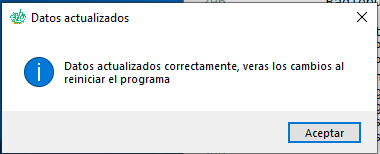
\includegraphics[scale=1]{Informacion} 
\caption{Ventana emergente de información}
\end{figure}
Muestra la información de que un proceso ha concluido correctamente. También explican si el usuario ha de realizar algo una vez terminado el proceso para que termine la completa finalización de este.\\


\textbf{Aviso}\\

\begin{figure}[ht]
\centering
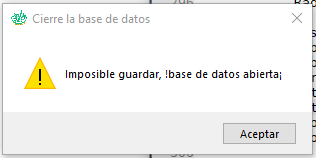
\includegraphics[scale=1]{Aviso} 
\caption{Ventana emergente que avisa que una acción no se ha podido realizar.}
\end{figure}
Pantalla que advierte que algo no ha salido bien. El usuario puede seguir con el uso del programa, pero si quiere realizar la acción que estaba realizando, deberá seguir las instrucciones proporcionadas en el cuadro de aviso.\\
\clearpage
\textbf{Error}\\

\begin{figure}[ht]
\centering
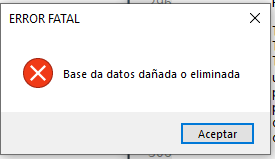
\includegraphics[scale=1]{Error} 
\caption{Ventana emergente que muestra que ha ocurrido un Error.}
\end{figure}
Pantalla que advierte de un error grave, en el que se ha corrompido la estructura de datos del programa.\\

A través de estos cuadros se traduce los diferentes problemas que puedan surgir en la utilización del programa; de manera gráfica y entendible por el usuario, haciendo el funcionamiento de este lo más transparente al usuario posible.
\subsection{Diseño}
Diseño simple, se evita crear extensos árboles de ventanas y frames, creando una navegabilidad sencilla e intuitiva. Debido al principal objetivo del proyecto,  esta aplicación está orientada a todos los públicos, por lo que se procura que la interfaz sea simplista, y fácil de entender.\\

Se basa en un menú principal ramificado en tres vertientes: Usuario, Dieta y Registro (en el programa aparecen con otros nombres). En la vertiente usuario, esta la información del usuario y la posibilidad de cambiar dichos datos para un avance del programa. En la rama de la dieta se encuentra el tronco principal de la aplicación, se muestra las recomendaciones alimenticias, a parte de darte libertad a la hora de escoger y decidir que deseas comer en el día de hoy. Por último estaría el registro o historial, es decir, todo aquello que necesites para llevar un registro de tu progreso y concienciar de esta manera al usuario.\\

Respecto a los colores, se decido un tema básico que no agote la vista del usuario, ni tenga múltiples colores deslumbrantes, da la posibilidad al usuario de elegir entre una serie de estilos predefinidos para que escoja el que mejor se ajuste a sus gustos y necesidades.\\
\section{Estructura del programa}
\subsection{Introducción}

La estructura es una variación del modelo-vista-controlador, separando el módulo HealthApp (que funciona de Main), del resto de módulos, que son los que implementan la estructura CAV (Cálculos, Administración y Vista).
\begin{enumerate}
\item	\textbf{HealthApp} – Tronco del programa
\item	\textbf{Vistas} – Relacionado con la parte visual
\item	\textbf{CalculosDieta} – Todo cálculo usado en el programa
\item	\textbf{AdminBase} – Todo proceso relacionado con la base de datos

\end{enumerate}

\subsection{Cálculos, Administración y vista}
Podríamos llamar propiamente a este modelo el CAV, y se basa en separar toda función que se vaya a crear en el programa en estos tres pilares. \\
Cada vez que la lógica de una función necesitaba un hueco donde encajar y ninguno de los módulos creados lo sostenía, se iba creando un nuevo módulo. Debido a la forma de trabajar del alumno, la estructura acabó cogiendo esta forma.  Por un lado, todo elemento relacionado con la base de datos, por otro lado todo cálculo matemático realizado en el programa y por último toda función que intervenga en la interacción usuario-aplicación.\\

Para crear una estructura, y no tener un código modular sin coherencia, se llevó a cabo una serie de reglas sencillas:
\begin{itemize}
\item	Si su finalidad es puramente visual – Vista
\item	Si realiza cálculos u operaciones matemáticas, indistintamente de si sea sobre la dieta -CalculosDieta
\item	Si interacciona y guarda datos en la base de datos -AdminBase
\item	Si mezcla alguna de estas funcionalidades, por ejemplo, guardar en la base de datos y mostrar por pantalla algo, se tendrá en cuenta cual es su principal finalidad, por ejemplo, se guardan estilos que se cargaran automáticamente para el diseño del programa, obviamente su finalidad es puramente visual, y guardar en la base de datos una transacción necesaria.
\item	Cualquier objeto, ventana, tabulación, etc. Que siempre vaya estar ahí al HealthApp, pero sus modificaciones se repartirán entre los diferentes módulos.

\end{itemize}
Estas reglas, a día de hoy, han cumplido con todas las funciones que se han creado en el programa dando el resultado previsto.
\section{Librerías}
\subsection{Pandas}
La librería desarrollada por Wes McKinney, Pandas, es una librería usada para el tratamiento de los datos como estructuras. Debido a que este proyecto se enfoca en el análisis de datos, y no en el tratamiento de bases de datos, se decidió crear una base de datos local en un archivo Excel.\\
La primera opción fue la librería “openpyxl”, la cual es una librería de código abierto, que permite la carga y manejo de datos ".XLS". De esta manera se  cargaba los datos, pero en listas desestructuradas que complicaban el posterior análisis de la información.\\
Acto seguido basándose en el libro: Python for Data Analysis \cite{analisis}, se decidió probar con Pandas, esta librería permitía leer los datos de los archivos ".xlsx", en forma de DataFrames. Simplificando el análisis de los datos, permitiendo tratarles tanto como DataFrames como en forma de vectores.
\subsection{Numpy}
Como se ha nombrado anteriormente, el libro: Python for Data Analysis \cite{analisis}; Hace especial énfasis en la conveniencia del uso de Numpy para el tratamiento y análisis de los datos. Es la principal librería sobre la que se ha  trabajado a lo largo de la carrera en cuanto a análisis de datos en Python, y una de las mas recomendadas por varias fuentes de información. La librería Numpy es la encargada, del tratamiento, procesamiento y cálculo de todos los datos que internamente realiza el programa.
\subsection{Interfaz Gráfica}
La librería utilizada para realizar y diseñar la interfaz gráfica fue Tkinter, tras indagar en diferentes fuentes, se decantó por Tkinter debido al desconocimiento sobre el funcionamiento de interfaces gráficas con Python. Entre las opciones que se barajaron se encontraban: Tkinter, WxPython, PyQt y PyGTK.\\

Tkinter presentaba una serie de ventajas: viene preinstalada con Python, es fácil de aprender y además cuenta con una documentación amplia y extensa. Pero entre sus desventajas, se encuentran: la escasez de recursos gráficos, la sencillez implica poca variedad de elementos y funciones (complicando en numerosas ocasiones la navegabilidad) y la lentitud que este tiene debido a que dibuja cada elemento sobre cada pantalla, en tiempo de ejecución.\\

La segunda opción que se planteo, fue WxPython. Presentaba  grandes ventajas como: la rapidez,  la flexibilidad que este ofrecía y la variedad opciones que tiene para crear una interfaz gráfica compleja. Después de ser meditado se llego a la conclusión de que todo lo que  ofrecía WxPython, era innecesario para la interfaz tan simplista que necesitaba el proyecto, y el aprendizaje era más complejo, además de tener recursos limitados, y tener menor cantidad de documentación al alcance del alumno. Su mayor inconveniente es que tiene una comunidad muy activa, la cual está constantemente insertando cambios y creando problemas de compatibilidad.\\

El resto de librerías fueron descartadas, al poco de buscar información sobre ellas puesto que daban las mismas ventajas o similares que la WxPython, pero tenían mas inconvenientes, al menos para el tema que aborda este proyecto.
\subsection{MatplotLib}
Librería de Python extendida en su uso, para el análisis y representación de los datos. Se utiliza a lo largo del proyecto para crear diferentes gráficos e histogramas para dar una perspectiva más visual de los resultados al usuario.
\subsection{Pillow}
Usada en su versión 6.0. Es una librería que permite la carga y posterior muestra de imágenes en una aplicación Python. Es usada en numerosas ocasiones a lo largo del proyecto, para visualizar el logotipo, o diferentes imágenes guía que ayudan al mejor entendimiento del programa.
\subsection{webbrowser}
Módulo que proviene de una interfaz de alto nivel para mostrar archivos web a los usuarios.
\subsection{os}
Librería utilizada durante el proyecto para la carga del manual en PDF por parte del programa. Es una librería cómoda que permite acceder y mostrar varios elementos que se encuentran en el sistema.
\subsection{datetime}
Librería normalmente preinstalada con Python, que da un control sobre la fecha y la hora del sistema. Sumamente útil para el control de registros  e historial.

\subsection{auto-py-to-exe}
No es usada durante el desarrollo del proyecto, pero si al finalizar dicho desarrollo para crear un archivo ejecutable (.exe). Utiliza internamente la librería pyinstaler, y hace uso de la librería Tkinter para otorgar una interfaz gráfica al comando pyinstaller, haciendo más fácil su uso.

\section{Módulos}
\subsection{Cálculos Dieta}
Módulo encargado de los cálculos del programa. En el se encuentra el motor del sistema de recomendación, encargándose de:
\begin{itemize}
\item Calcular la calidad de los alimentos en base a sus características.(Algoritmo Nutriscore)
\item Calculo y reajuste de la Tasa Metabólica Basal (TMB)
\item Reparto de kilocalorías y los diferentes macronutrientes, teniendo en cuenta la comida del día y las necesidades que este aplica.
\item Aplicación de la formula del sistema de recomendación
\end{itemize}

\subsubsection{Reparto Calórico entre comidas.}
Como se aprecia en la Tabla \ref{tabla:porcentaje}, se tiene en cuenta no solo la carga calórica en cada comida, sino la distribución de este porcentaje entre los distintos nutrientes. (Consultar Tabla \ref{tabla:distribucionDietas})\\

\tablaSmall{Porcentajes totales de cada comida}{l c c c c}{porcentaje}
{ \multicolumn{1}{l}{Comida } & Porcentaje(\%) & Descripción\\}{ 
Desayuno & 24,75 & Alta carga calórica, rica en hidratos\\
Almuerzo & 13,5 & Baja carga calórica.\\
Comida & 30,5 & Mayor carga calórica, eje central.\\
Merienda & 11,5 & comida de paso y casi prescindible.\\
Cena & 19,75 & Alta carga calórica pero con moderación.\\
} 
Se calcula el número de Kilocalorías que se tiene que tomar de hidratos, grasas y proteínas, en base al tipo de dieta recomendable para su patología.\textbf{distribuciónDeMacronutrientes} toma como parámetros las kilocalorías diarias calculadas previamente por la función calculoTMB, y el tipo de dieta del usuario en base a su patología, y te devuelve una lista de los macronutrientes diarios, repartidos en gramos y las kilocalorías totales en el siguiente orden: ListMacDiarios [Kilocalorías, Hidratos, Proteínas, Grasas].

\subsubsection{Formula del Sistema de recomendación}
Motor del sistema de recomendación. A través de la formula:
\begin{equation}
DiferenciaMacronutriente = \frac{(KMCD - A)}{((KCDT-KMM)+(KMTC-KTM))}
\end{equation}
Donde:
\begin{itemize}
\item \textbf{KMCD:} Número de Kicalorías del macronutriente (Hidratos, proteínas o grasas) de la Comida (Desayuno, almuerzo...) que debería llevar en esa comida
\item \textbf{A:} Actual número de kicalorías de ese macronuetriente que llevo en todo el día (Si estoy en Comida: desayuno+almuerzo+comida).
\item \textbf{KCDT:} Kilocalorías que debería comer en esta comida concreta para este macronutriente concreto.
\item \textbf{KMM:} Kilocalorías del macronutriente concreto del menú.
\item \textbf{KMTC:} Kilocalorías totales que debería comer en esta comida.
\item \textbf{KTM:} Kilocalorías totales que tiene el menú a recomendar.

\end{itemize}
La fórmula es el eje central del filtro de recomendación basado en contenidos. Se evalúan diferentes características de los tres aspectos claves a la hora de la recomendación según este proyecto: Usuario, Alimento, y el momento del día.\\
De esta manera cuanto mayor sea la diferencia entre lo que debo llevar y lo que llevo comido, y menor sea la diferencia entre lo que deseo y las características del alimento, mayor será la puntuación de ese alimento para su recomendación ( \textbf{Nota: Se ordena de mayor diferencia a menor}).\\
Por último, se realiza la media entre los tres macronutrientes principales:
\begin{equation}
DiferenciaTotal = \frac{(Diff.Hidratos+Diff.Proteina+Diff.Grasas)}{3}
\end{equation} 
En el caso de que algún macronutriente dé negativo, no se tendrá en cuenta.


\subsection{AdminBase y estructura de la base de datos}
En este apartado se expone la estructura la base de datos y de como se cargan, guardan y trabajan los datos desde el módulo \textbf{AdminBase}, el cual, es el encargado del manejo de los datos, y la traducción con el sistema de archivos.
\subsubsection{CargaBaseDeDatos y guardaDatos}
Estas dos funciones cargan y guardan los datos de/en la base de datos respectivamente. Nada más iniciar la ejecución del programa, almacena los datos leídos de la base de datos, en una serie de DataFrames independientes. Se trabaja con cada uno de ellos sin tener en cuenta al resto y se guarda el resultado de los cambios producidos durante la ejecución del programa, sustituyendo la base de datos por los DataFrames. \\

\subsubsection{Estructura de la base de datos}
La base de datos es almacenada en diversas hojas de cálculo, simulando de esta manera diferentes colecciones de una base de datos. Estas colecciones serias:\\
\textbf{\textsc{ALIMENTOS}}\\
La hoja de alimentos, es una hoja de menús ya construidos. Esta hoja consta de doce campos:\\
La clave primaria de esta colección es el nombre del menú. Los campos son:
\imagen{A}{Estructura base de datos alimentos}
Nombre (Único), Calorías, Grasa, Saturadas, Hidratos, Fibra, Azúcares, Proteínas, Sodio, Tipo, LRE(Last Reciently Eat) y Calidad.
Los primeros diez campos son las diferentes características del menú, mientras que los otros tres son parte de la gestión de dichos menús.\\
El tipo marca el tipo de comida que es, un mismo menú puede ser a la vez desayuno, almuerzo y merienda, cena y comida, etcétera. Por ello se planteo dos posibilidades.
\begin{enumerate}
\item Cadena de carácteres, con la combinación de la inicial o nombre de las diferentes combinaciones de tipos de comida y la posterior separación de estas. Esto dio diversos problemas con la carga y filtrado de los datos.
\item Cadena de bits: desayuno-almuerzo-comida-merienda-cena, donde el valor 1 sería si es valido para esa comida y 0 si no lo es.
\end{enumerate} 
Se decidió escoger la segunda opción. Una vez creado los métodos que traducen el sistema numérico en una cadena de bits, el tratamiento en conjunto de las combinaciones como un simple número simplificó las cosas. Ejemplo:
1-1-0-1-0 \\
Significa que es desayuno, almuerzo y merienda, pero no comida o cena, luego esto se traduce en el número decimal, que en este caso sería 26.\\

El LRE lleva una métrica de la frecuencia con la que el usuario toma esa opción, literalmente significa “last reciently eat” (El más reciente ingerido), que en este caso hará de contador. En la expansión del proyecto (Explicado en el apartado 7), este dato sería el único encontrado de manera Local, ayudando a personalizar aún más la aplicación para una mejor experiencia de usuario. \\

La Calidad, como el propio nombre indica, es la calidad del alimento, es la variable que marca la diferencia entre 100 kilocalorías de ensalada y 100 kilocalorías de azúcar. Tiene un rango de valores de la A a la E, siendo A una comida saludable, y E una comida poco recomendable. Internamente el programa lo trata de forma numérica. Este valor se halla a través del algoritmo Nutriscore.

\textbf{\textsc{Usuarios}}\\
La hoja de usuarios alberga los datos de todos los usuarios que usan la aplicación. Está estructurada de forma que contenga los datos principales del usuario, así como, los datos necesarios para el sistema de recomendación. \\
\imagen{BaseUsuarios}{Estructura base de datos Usuarios}
La clave primaria sería el DNI del usuario, el cual, se encuentra dentro del campo ID. La hoja se estructura de la siguiente manera:\\
Id (PK)-nombre-apellido-password-sexo-edad-altura-peso-actividad-patología (FK de la tabla Patologías) y tipo.\\
Tanto \textbf{id, como nombre, apellido y password}, son los datos privados del usuario, los cuales, son simplemente informativos y no tienen ningún valor adicional en el cálculo de la dieta y los resultados. En cambio, \textbf{el sexo, la edad, altura, peso, actividad, patología y tipo, influyen de manera directa con el cálculo de la dieta} . A tener en cuenta, que el valor del campo patología es numérico para mayor privacidad y conexión con la base de datos de Patologías, pues es el id de cada patología. En el caso de valer -1, significa que el usuario no tiene ningún tipo de patología y su uso es exclusivamente para el aprendizaje y seguimiento de la dietoterapia adecuada. La actividad tiene valores entre 0 y 4, donde cero significa el máximo nivel de sedentarismo y 4 el máximo nivel de actividad. Por último el tipo, hace referencia, a los objetivos que el usuario tiene respecto a si mismo, si quiere mantenerse, subir de peso, o bajar.\\

\textbf{\textsc{Patologías}}\\
En esta hoja, la cual se encuentra dentro de las BaseDeDatosDeAlimentos, está la información básica de las patologías: \textbf{nombre}, \textbf{id}, y el \textbf{tipo} de dieta que lleva alto o bajo en carbohidratos, proteínas o grasas. Esto se carga al inicio del programa, se comprueba si el usuario padece alguna patología y se selecciona el tipo de dieta correspondiente.\\
\begin{figure}[htb]
\centering
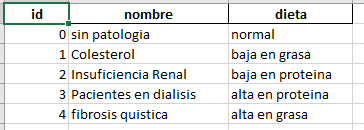
\includegraphics[scale=1]{Patologia} 
\caption{Estructura base de datos Patologías}
\end{figure}

\textbf{\textsc{Registro}}\\
Base de datos que se encuentra en la ruta: assets/RegistroMejora.xlsx, y se encarga de llevar un registro de la mejora del usuario en la aplicación. Esta base de datos guarda los datos imprescindibles para el ajuste de la formula del TMB respecto al usuario concreto.\\
En el momento que un usuario se registra, tiene tres posibilidades de tipo de dieta:
\begin{enumerate}
\item \textbf{bajar:} Se crea un valor inicial igual a -500
\item \textbf{Mantener:} Se crea un valor inicial igual a 0
\item \textbf{Subir:} Se crea un valor inicial igual a 500. 
\end{enumerate}
El valor inicial a la hora del registro es el suplemento que se añade al resultado de la formula del metabolismo basal, para que las calorías a ingerir por el usuario sean las necesarias para lograr el objetivo que se ha propuesto a través del tipo de dieta.
Esta base de datos se estructura de la siguiente manera:
\begin{figure}[htb]
\centering
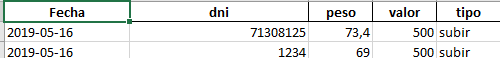
\includegraphics[scale=1]{registroMejora} 
\caption{Estructura base de datos Registro}
\end{figure}
Esto se debe a:
\begin{enumerate}
\item \textbf{Fecha:} Guarda la última vez que se editó la información. De esta manera se puede calcular el peso que se debería haber progresado hasta dicha fecha. No admite cambios de menos de una semana, pues el resultado podría alterar el ajuste del valor.
\item \textbf{dni:} DNI del usuario para saber de quién es el registro que se está llevando.
\item \textbf{Peso:} El peso de la última vez que el usuario edito la información respectiva a su peso. Esto ayuda al seguimiento de la dieta y sus objetivos.
\item \textbf{Valor:} Valor que más tarde se suma al cálculo TMB y que ayuda a cumplimentar mejor su objetivo.
\item \textbf{tipo:} Tipo de dieta u objetivo de la dieta del usuario. Sirve para saber si el usuario a cambiado de objetivo y en caso de no hacerlo, ver cómo va el progreso del usuario.
\end{enumerate}

\subsection{Vista}
En el módulo vista se almacena toda función que tendrá influencia en lo que el usuario ve, es decir:
\begin{enumerate}
\item Actualización de pantallas,
\item Muestra de datos,
\item Transacciones entre ventanas,
\item Actualización de los gráficos,
\item Etcétera.
\end{enumerate} 


\subsubsection{Reconstrucción de frames}

Cada vez que se selecciona una opción, el resto de las opciones cambian aplicándose el sistema de recomendación programado. Se van ajustando las opciones a las necesidades del usuario. Tkinter no dispone de ningún método eficaz que permitiese actualizar un Frame. Por ello, cada vez que se selecciona una opción, se crea un nuevo frame que sustituye al actual, llamándose de manera recursiva con distintas opciones sobre el sistema de recomendación.\\

Para evitar errores de coherencia el programa solo actualizará aquellos Frames no bloqueados por el método seleccionar, sacrificando un pequeño porcentaje de la precisión, para conseguir un funcionamiento más fluido sin errores de compatibilidad o múltiples selecciones.\\
\subsection{HealthApp}
Es la columna vertebral del programa, el cual, se encarga de cargar y procesar toda la información relevante que más adelante se va a ir editando en el programa. HealthApp tiene una única función y el resto se divide en clases que se instancian en esta función.\\

Hace de flujo de entrada y salida, donde una condición simula un interruptor permitiendo que la aplicación original, distribuida en clases, se lance o se cierre.\\

Todo se basa en una  jerarquía de objetos, en el que el objeto principal (Menú principal), contiene otros tres objetos que estos a su vez contienen otros, creando una simple estructura de árbol, entendible por cualquier programador. \\

Se crea una clase por tipo de comida barajada. Por lo que cada vez que se crea de manera recursiva el mismo Frame, se está instanciando la clase contenida.

\section{Herramientas}
 Nos centraremos en mencionar de manera breve, las herramientas que se han usado para el desarrollo del programa.
\subsubsection{Anaconda}
Distribución de código abierto, la cual, está indicada para el análisis, procesamiento y computo de datos, de Python y R, trae consigo una serie de programas y características entre los que destacaremos: Spyder y VisualCode.\\

Se decidió usar anaconda, debido a su principal función, el análisis, procesamiento y computo de los datos.
\subsubsection{Spyder}
Spyder es un entorno de desarrollo incluido en el paquete de anaconda.\\

Antes de empezar se probaron varios entornos como: NoteBook, PyCharm, VisualCode y eclipse (añadiendo el API de Python), pero se acabó decantando por Spyder.\\

\subsubsection{GitHub}
Proyección de la metodología GIT para el almacenamiento y control de versiones, sin duda GIT es actualmente la estructura más usada en el mundo de la programación, y GitHub, una de las herramientas más conocidas y valoradas que hay.
\subsubsection{GitKraken}
Potente interfaz gráfica multiplataforma desarrollada por Electron, que nos permite controlar de forma sencilla y cómoda nuestro repositorio GitHub, permitiendo que el uso y control del GitHub fuera más ameno y rápido, sin duda es una de las mejores aplicaciones que he probado, y de las que más me han ayudado a lo largo del proyecto.
\subsubsection{MakeText}
Herramienta de escritorio, utilizada para la preparación de documentos en LaTex. Fue utilizada durante el desarrollo del proyecto para plasmar las memorias y anexos, que formarían la documentación del proyecto.
\capitulo{5}{Aspectos relevantes del desarrollo del proyecto}

\section{La idea}
Uno de los aspectos a destacar en el desarrollo de este proyecto, es el nacimiento de dicho proyecto. Se trata de un trabajo de fin de grado, el cual, es un trabajo puro del alumno, donde tanto idea como desarrollo son realizados por él. Una parte del tiempo gastado en el desarrollo fue en la ocurrencia y el pulimento de la idea. Aunque dicha idea fuera cambiando a lo largo de su desarrollo.\\

La necesidad de hacer alfo interesante, diferente y que fuera un tema de actualidad, son los pilares sobre los que se sustenta la idea. Para ello, se llevo a cabo una investigación sobre de las necesidades que sufren las personas hoy en día, con las ultimas corrientes de moda y que además pudiera resultar útil. La salud y la buena calidad de vida, son temas de vital importancia para las personas, que con el paso del tiempo cobran cada vez más protagonismo.\\

Una vez encontrado el groso del proyecto tocaba perfilar detalles, para ver a través de que medio se podía llevar “una mejor calidad de vida” al usuario. De aquí surgieron varias vertientes:\\

\begin{itemize}
\item	Deporte: Descartad, por la inmensa cantidad de aplicaciones de planificación de entrenamiento que existes a día de hoy.
\item	Nutrición: Inicialmente descartada, debido a las mismas razones que lo anterior, existen cientos de aplicaciones tanto que te proponen una dieta como que te ayudan a seguirla.
\item	Recordatorios: Con esto me refiero, a recordatorios de cuando hacer deporte, de cuando tomarse los medicamentes, etc. Se descarto rápidamente por ser una más, a la par que un proyecto banal.
\item	Nutrición con otro enfoque: Aquí es donde llego la idea, una vez descartadas las demás opciones. Se ideo  una aplicación que te enseñe a comer, y que tenga en cuenta las patologías aunque sean en menor medida. Ahí es cuando nació la idea, y se empezó a formar la idea de la estructura de lo que iba a ser el proyecto.

\end{itemize}
De este modo se empezó con el proyecto, partiendo totalmente de cero, hasta el punto de conseguir algo perfectamente funcional, cumplimentando los objetivos propuestos para dicho proyecto.

\section{Formato de trabajo}
Se desarrollo una metodología ágil de forma incremental. Se empezó formalizando las bases hasta llegar a la etapa final. No se pasó a la siguiente etapa sin haber terminado la anterior.\\

Las tres principales etapas del proyecto fueron:
\begin{enumerate}
\item	Funcionamiento por interfaz Shell
\item	Funcionamiento de manera gráfica
\item	Finalización de cada detalle dejado indicado durante el proyecto.
\end{enumerate}

De esta forma, se fueron creando todas las características de manera progresiva, de forma que se dio mas importancia al claro desarrollo del proyecto, que a la velocidad de dicho desarrollo. Debido al sistema de organización por etapas, se logra un desarrollo fluido. Utilizando los recursos substraídos de la etapa anterior, impidiendo parches en el código o incoherencias.\\

Se desarrollo en estas tres etapas principales debido a los conocimientos del alumno. Desarrollar primero una aplicación por interfaz de comandos, permitió desarrollar el motor de la aplicación, sin tener que preocuparse por otro tipo de problemas, esto permitió crear una estructura solida, que posteriormente heredaría la fase de la interfaz gráfica.\\

\section{Algoritmos del programa}
Se desarrollan desde cero una serie de algoritmos o sistemas de tratamiento de los datos. Haciendo de esta parte algo propio de este proyecto.
\subsection{Algoritmos de recomendación}
Es el algoritmo que estructura todo el sistema de recomendación, nace de la necesidad de que la recomendación se ajuste al máximo a las necesidades del usuario.\\
Si se ordenaba única y exclusivamente por la calidad, nunca se verían los menús de peor calidad, y el usuario nunca aprendería a llevar un estilo de vida saludable; además de que podría haber una desigualdad inmensa entre las calorías ingeridas y las necesitadas.\\
Se pensó en hacer una formula basada en la diferencia calórica, cosa que se adecuaba mas a las necesidades del usuario, pero creaba un desajuste en los macronutrientes, rompiendo la idea de dieta equilibrada. Por ello, se ideo otro prototipo de formula.\\

La formula tiene en cuenta la proporción de las necesidades calóricas del usuario, partiendo de cada macronutriente, se calcula la diferencia entre la diferencia de macronutrientes que debería llevar y los que llevo, todo llevo partido por la suma de la diferencia entre: Las kilocalorías que debo comer y las que tiene el alimento y la diferencia entre el macronutriente especifico y lo que el alimento tiene.\\
\begin{equation}
DiferenciaMacronutriente = \frac{(KMCD - A)}{((KCDT-KMM)+(KMTC-KTM))}
\end{equation}
Donde:
\begin{itemize}
\item \textbf{KMCD:} Número de Kcalorias del macronutriente (Hidratos,proteinas o grasas) de la Comida (Desayuno, almuerzo...) que debería llevar en esa comida
\item \textbf{A:} Actual número de kcalorias de ese macronuetriente que llevo en todo el día (Si estoy en Comida: desayuno+almuerzo+comida).
\item \textbf{KCDT:} Kilocalorias que debería comer en esta comida concreta para este macronutriente concreto.
\item \textbf{KMM:} Kilocalorias del macronutriente concreto del menú.
\item \textbf{KMTC:} Kilocalorias totales que debería comer en esta comida.
\item \textbf{ktm:} kilocalorias totales que tiene el menú a recomendar.
\end{itemize}

\subsection{Reajuste del TMB}
Durante el proyecto, se usa la formula para el calculo del Metabolismo Basal, esto da como resultado las calorías que el usuario consume en un día normal. A esta cantidad de calorías se le suele variar un cantidad de calorías que suele oscilar entre las 300 y 500 calorías. Para poder bajar o subir de peso de manera controlada (Aproximadamente 3 kilogramos al mes). Esta formula antiguamente estaba muy extendida entre nutricionistas y endocrinos a la hora de diagnosticar/proporcionar una dieta. Con los años, entro en desuso, debido a la generalidad que hacer la formula sobre las calorías que gasta cada persona, sin tener en cuenta metabolismos, posibles enfermedades, etcétera.\\

Desde el principio fue un problema que limitaba las posibilidades del proyecto. Por ello, se desarrolló un método que permite, a través de una coleccióm de registros, llevar la cuenta de las variaciones de peso que sufre el usuario, y amoldar ese valor fijo, permitiendo su reajuste, y creando una formula que se adapta con mayor precisión a las necesidades del usuario.\\

\subsection{Persistencia de los datos}
No es propiamente un algoritmo, sino  un recurso para solucionar una de las mayores limitaciones que presentaba usar una hoja de calculo como base de datos y evitar  datos sobre-escritos y problemas con los datos. Se procuró durante todo el programa atomizar al máximo posible cada método sobre la base de datos, haciendo que los cambios sean lo mas inconexos y manejables para el usuario. \\

En el método añadir alimento se rompe esta norma, añadiendo un alimento en la base de datos que hay que guardar, pero sin guardar todos los cambios en el resto de los alimentos, por si el usuario no quisiera hacerlo. Para evitar esta falta de control por parte del usuario sobre la persistencia de sus datos, a la hora de almacenarlo, se carga el array de nuevo, y se añade esta nueva línea tanto al array usado durante el programa, como al nuevo array de alimentos, este nuevo array se almacena en la base de datos, mientras que el otro sigue con su propósito en el programa. Si el usuario hace algún cambio y lo guarda, el nuevo alimento estará a salvo, si, por el contrario, el usuario decide salir sin guardar su progreso en el día, el nuevo alimento ya estará guardado en la base de datos.\\
\subsection{Distinción entre tipos de comida}
Uno de los retos a afrontar a lo largo de este proyecto fue simplemente, el como se iba a indicar que tipo de comida/menú era. Sin duda no fue uno de los retos más complejos abordados a lo largo del proyecto, pero si uno de los más curiosos.\\

Recordamos que un mismo menú, puede pertenecer a varias comidas del día, entonces se pensaron varios métodos hasta llegar al óptimo, los cuales explicaremos con brevedad a continuación:\\

Se realizó un estudio sobre los diferentes métodos de distinción que se podían realizar. Se pensó en  cadenas de caracteres (String) separadas por un delimitador cualquiera, y cargarlo en forma de cadena de caracteres separandolo utilizando algún delimitador (Por ejemplo Slice() y delimitador ':'), pero esto provocó ciertos problemas de carga y almacenamiento, problemas no demasiados complejos, pero que aumentaban la complejidad algoritmo al buscar a través de un bucle todas las posibilidades complicando esto, y se pensó en una concatenación de bits donde 1 es que era esa comida y 0 que no, es decir: 11010, Significa que no es ni comida ni cena. Esto presentaba el mismo problema que la cadena de caracteres y era quizás más confuso para su compresión, Además del pequeño inconveniente de que si un menú no era desayuno ( Es decir empezaba en 0), en algunas ocasiones se almacenaba sin ese digito creando una desigualdad en el programa. Por estas razones se deicidio pasar al siguiente método, una mezcla de ambas, se iba a usar una cadena para calcular un único valor que cargar. Finalmente se paso esa cadena de bits a un valor numérico, de esta manera se asegura una única carga, y el tratamiento a través de cláusulas condicionales simples.\\

\textbf{Ejemplo:}\\
Un alimento que sea comida y cena: 00101 -> Se representará con el número 5. \\
Esto permite la carga de un único elemento, sin posibilidad de fallo además de un calculo sencillo, cuyo mayor inconveniente es llevar a cabo todas las clausulas condicionales, para hacer la criba por tipo de comida.\\

\section{Conocimientos aprendidos en la carrera}
\subsection{INTRODUCCIÓN}
Apartado donde se hablará de forma breve sobre todo conocimiento aprendido durante los años de carrera, relacionado directamente con el desarrollo del proyecto.
\subsection{Conocimientos sobre python}
A lo largo de la carrera, se han estudiado diferentes lenguajes de programación (Ej: Java, C, CSHARP...), entre los cuales se encontraba Python. Por ejemplo en asignaturas como Sistemas Inteligentes, Nuevas tecnologías, etc., o vistas también en la  politécnica de Varsovia, en asignaturas como “Algoritmia y computación matemática”.\\

Además, varias de las librerías usadas durante este proyecto fueron utilizadas en dichas asignaturas, haciendo que el proyecto, partiera desde un punto avanzado facilitándome el aprendizaje.
\subsection{SCRUM}
Quizás uno de los aspectos más destacados a la hora de realizar el proyecto, fue la organización por parte del alumno, a través de la metodología SCRUM, que permitía al alumno mantenerse centrado en cada nueva tarea, no pasando a la siguiente hasta dejar esta zanjada del todo. \\

Para la realización del proyecto, se usa una pizarra física, donde se colocan las diferentes tareas, con una fecha limite de realización, de esta manera, toda idea que se planteaba durante el desarrollo era plasmada en la pizarra y posteriormente hecha. \\
La pizarra era dividida en cuatro partes (pequeña adaptación del SCRUM).\\
\begin{enumerate}
\item	TODO: Por hacer, eran todas las tareas, pautas, e ideas que iban surgiendo a lo largo de la semana o tras las reuniones semanales. Había un máximo de cinco, para evitar que el proyecto se atascase por una carga excesiva de trabajo. De TODO se pasaba a in progress. 
\item	IN-PROGRESS: En proceso, máximo dos cosas, una principal y una secundaria, la principal, consistía en el desarrollo de grandes métodos, cálculos, etc. Mientras que los secundarios, podían ser trabajos de investigación, rellenar datos o cualquier detalle que faltase de completas. De esta manera se evitaba la bifurcación del trabajo, haciendo del camino, pequeños objetivos, claros y directos a completar. Cuando el alumno pensaba que había terminado la tarea, la movía a “TO-VERIFY”.
\item	TO-VERIFY: A verificar, es decir, falta la aprobación de los cambios realizados, si eran cambios propuestos en las reuniones semanales, eran zanjados en la siguiente reunión semanal; De esta forma se creaban distintos modelos y versiones de métodos, perfilando al máximo cada detalle en cada método. Las pequeñas tareas, eran resueltas, ya fuera en las reuniones semanales, o preguntando a personas, sobre como sería para ellos el correcto funcionamiento del programa.
\item	DONE: Una vez todas las partes se ponían de acuerdo en que la tarea estaba terminada, pasaban a DONE, este apartado existía básicamente, para hacer mella en el trabajo que el alumno realizó durante la semana, haciendo palpable las semanas donde se tuvo una mayor o menor carga de trabajo, pudiendo regular esto, y teniendo de esta manera un avance constante.
\end{enumerate}
En progreso solo se podía encontrar una tarea, y si el tutor catalogaba una tarea ya en "TO-VERIFY" como incompleta pasaba de nuevo a "In progress" de manera que, de esta forma, semanalmente se cumplían con una serie de propósitos de forma clara y concisa, y no se aglomeraban todas las ideas y propuestas dejando  cabos sueltos que podrían arruinar la representación final del proyecto. \\
Este método fue estudiado en la asignatura de gestión de proyectos por el alumno, y culminado en su periodo de practicas con el instituto de Castilla y León, el cual, usaban de manera muy similar a la adaptación del alumno, La metodología SCRUM para gestionar todos sus proyectos.\\

\subsection{Investigación}
De vital importancia es el nivel de capacidad de investigación y búsqueda de la información La velocidad y capacidad, de saber buscar, es uno de los conocimientos más importantes que se adquieren a lo largo de la carrera. Conocimiento indirecto, pero presente en todas y cada una de las asignaturas que se han cursado, dicho nivel de investigación permite verificar de forma mas precisa, tanto  los datos o recursos necesarios para una investigación como la solución de errores que puedan emerger durante el desarrollo.
\section{Conocimientos externos a la carrera}
\subsection{INTRODUCCIÓN}
En este apartado, se explicarán los aspectos relevantes del desarrollo del proyecto externos a los conocimientos iniciales del alumno. Todo aquello que ha tenido que aprender para poder llegar al resultado final.
\subsection{Psicología}
Parte de psicología, intercalada con  parte de educación primaria. Para el desarrollo del proyecto, y el moldeado de lo que es la idea genérica de este; Ha sido necesario el estudio de ciertos campos para entender cual podría ser el mejor camino para el entendimiento con el usuario. Este proyecto no buscaba una forma rápida de llegar al cliente/usuario, sino constante, que el cliente convierta los cimientos de la aplicación, en su propio estilo de vida. Por ello se estudió las distintas formas de enseñanza, así como, el auge de la tecnología en el sistema educativo.
\subsubsection{Aprender a aprender \cite{autoAprendizajeForma}}
Usado en la educación primaria e infantil, es un método para enseñar al alumno, en base a que el alumno encuentre la propia respuesta. De esta manera desarrolla los estímulos positivos del alumno ante la adquisición de nuevos conocimientos. \\
La idea principal nace de las ventajas que tiene implementar un estilo de vida, sobre el seguir ordenes estrictas. Tras un periodo de investigación, se decanto por un estilo progresivo, en el que se intenta concienciar al usuario de cada decisión que toma, haciendo que el aprendizaje se base en pequeñas metas personales, y en la concienciación del usuario para que, él mismo, se de cuenta de que es lo mejor para él y aunque de manera lenta pero segura, llegue a la meta que tenga como objetivo.
\subsection{Nutrición}
Conocimientos básicos sobre el mundo de la nutrición, el reparto da los distintos nutrientes de cada alimento a lo largo del día y la correcta distribución de las calorías en base a las características del usuario.\\

Para el desarrollo del proyecto, se ha necesitado conocimientos sobre la calidad de los alimentos, así como, la predisposición de cada tipo de patología en base a las características de los alimentos. Logrando, a través del estudio e investigación, un análisis detallado para la veracidad de los datos a tratar.
\subsubsection{"Calidad" de los alimentos}
Parte fundamental del proyecto, la calidad marca el umbral por el cual se cribaran los alimentos y se aconsejarán principalmente los alimentos de mejor calidad, y esto irá variando conforme a que  el usuario busque nuevos alimentos, u opciones.
\subsection{Nutriscore}
Algoritmo del semáforo o NUTRISCORE, algoritmo que se basa en una serie de características buenas y malas de los alimentos, y según el resultado de la diferencia, la cual, se acaba cribando en uno de los cinco posibles valores: A,B,C,D Y E, ordenador de mejor a peor.\\

\imagen{Nutriscore}{Algoritmo nutriscore}

Con este algoritmo se logra una integridad de los datos en la base de datos, pese a que el usuario añada sus propios alimentos. Para hallar la calidad del menú completo se usa una pequeña variación del algoritmo en cuestión para tratar diferentes alimentos con diferentes calidades.
\subsubsection{Imperfecciones}
Este algoritmo contiene fallos, pues se basa única y exclusivamente en cifras, en las cifras de azúcar, de proteína, de sal, etc. Por lo cual, cosas saludables como puede ser el aceite de oliva virgen extra, tienen como resultado una pésima calidad, mientras que, quizás, ultraprocesados como cereales bajos en azucares, bebidas edulcoradas y cosas de gran similitud nutricional, adquieren una buena calidad. \\
Esto se debe por ejemplo, a que por cada 100 gramos, el aceite de oliva tiene una alto contenido en kilojulios y en grasas, por lo cual lo coloca en la categoría E, cuando debería ser un A.
\subsection{Interfaces Gráficas}
Pese a tener los conocimientos sobre programación en Python, se desconocía cualquier tipo de implementación de interfaz gráfica. Debido a esto, gran parte del  del proceso, fue la selección de la librería que se utilizaría durante el resto del proyecto para la implementación de este.\\
Finalmente se escogió Tkinter, por su sencillez, pues permitió dar grandes avances y adaptarse a este nuevo sistema rápidamente. Permitiendo que la interfaz se complicará de manera exponencial, aplicando todo aquello que se iba aprendiendo de manera colateral a lo ya existente.
\section{Fases del proyecto}
Las fases de este proyecto pueden ser divididas de diferentes modos, según que criterio se utilice, de por si podemos dividir todo el proyecto en tres grandes fases: Idea, desarrollo y testing. Teniendo en cuenta esto, hay que tener en cuenta que el desarrollo a su vez, se dividió en otras tres fases principales que fueron: creación de estructuras iniciales, desarrollo en interfaz de comandos y desarrollo en interfaz gráfica. 
Por lo cual un breve esquema del desarrollo podría ser:
\begin{itemize}
\item Nacimiento y pulimento de la idea
\item Desarrollo:
\begin{itemize}
\item Creación de la estructura de los datos.
\item Carga y manejo de los datos
\item Creación del proyecto por interfaz de comando
\item Traducción del proyecto a interfaz gráfica
\item Pulimento de detalles y nuevas funcionalidades
\end{itemize}
\item Pruebas
\item Desarrollo de la documentación pertinente
\end{itemize}
\subsection{Cronograma: }
\imagen{cronograma}{Tabla cronograma al completo}
\capitulo{6}{Trabajos relacionados}

El mundo de la dieta como terapia para el tratamiento de distintas patologías se investiga desde hace años, tomando día a día mas fuerza e importancia. Al principio se pensaba que la dieta solo era efectiva para las patologías cuya causa estaba estrictamente vinculada a la alimentación del paciente como es el caso de la diabetes. Con los años se fue fundamentando que se podrían prevenir otros tipos de enfermedades con una buena alimentación, como era el caso de los problemas cardiovasculares, la Osteoporosis e incluso el Cancer. En la actualidad, numerosos estudios defienden que una adecuada alimentación no solo ayuda a prevenir y tratar enfermedades relacionadas con la alimentación, sino que es una parte fundamental del tratamiento y/o recuperación de enfermedades tanto livianas como importantes, como son la Obesidad, el Cancer, y la esclerosis múltiple.
\section{Estudios:} 
\label{estudios}
\subsection{Estudios DASH} 
Los estudios DASH (Dietary Approaches to Stop Hypertension), son una serie de estudios relacionados para frenar la hipertensión a través una correcta alimentación, el primero de estos estudios se realizó en 1997. Realizado por la asociación del corazón americano (American Heart Association), el colegio americano de cardiología (American College of Cardiology), la sociedad contra el cancer americano y muchas otros colegios y universidades.\\

A grandes rasgos se basa en la relación directamente proporcional entre comer una dieta rica en frutas y verduras y baja en azucares, grasas y carnes rojas reduce terriblemente la hipertensión y las enfermedades relacionadas con el corazón.\\
\subsection{Las pruebas de grasas saturadas}
Son una serie de estudios, que se basan en demostrar la correlación entre las grasas saturadas y el incremento de factores de riesgo en enfermedades relacionadas con el corazón.
Pronto se observo en estudios como: https://www.sevencountriesstudy.com/ del que hablaremos más adelante, que la calidad de vida de las personas cuya alimentación era alta en grasas saturadas era bastante peor, teniendo una tendencia superior al padecimiento de enfermedades cardiovaculares.\\
\begin{quote}
By 1965 at the latest, it was beyond a reasonable doubt that if you replace saturated fats with polyunsaturated fats, you get a substantial lowering of total cholesterol. por Katan

(Traducción: En 1965 se probo que si se remplazan las grasas saturadas por polinsaturadas se obtiene un decremento del colesterol total.)
\end{quote}

\subsection{El programa de prevención de diabetes (DPP)}
Actualmente uno de cada tres adultos tiene diabetes, lo más significativo es que 9 de cada 10 no lo saben. \\

Los resultados del DPP, se basaron en una prueba asignada de manera aleatoria a 3234 personas con diabetes que tomaron placebos,  metformina (Una droga que baja el azúcar en sangre), o un “estilo de vida”.\\

La meta del estilo de vida consistía en perder peso y hacer ejercicio por lo menos dos horas y media a la semana.
Para el momento en el que se realizaron fue un resultado increíble ver que el medicamente aumentaba en un 31 por ciento el riesgo de diabetes, mientras que el estilo de vida lo reducía en un 27 por ciento. Un estilo de vida había superado con creces los resultados del medicamente. \\

\subsection{Pounds Lost}
Estudio basado en la perdida de peso, este estudio se realizó en 2004, y es uno de los estudios mas largos sobre la dietoterapia realizados hasta la fecha. Consistía en observar entre 800 personas, que macronutriente habría que reducir para mejorar el estado físico y la salud, si grasas, proteínas o carbohidratos.\\

Fue un estudio que se realizó durante dos años, y se observo que los sujetos a observación habían adelgazado prácticamente lo mismo, y ninguno sufría ninguna deficiencia notable que indicase que un macronutriente era mas necesario que otro.\\

Se esperaba que las personas con una dieta baja en carbohidratos y con resistencia a la insulina obtuvieran mejores resultados, pero no fue así.\\
Entonces se llegó a la conclusión de que era porque todos estaban comiendo saludable, sin azucares añadidos o hidratos refinados. Por lo que se demuestra que es increíble los avances que puede hacer la humanidad con una buena alimentación.
\subsection{Seven countries Study}
Fue el primer gran estudio que se realizó para relacionar la calidad de vida con la dieta y los posibles factores de riesgo que podría tener una mala alimentación sobre la salud de las personas.\\
Nació en dos partes, primero se realizaron estudios en Italia, España, Sudáfrica y Japón de 1952 a 1956 y se sugirió, que los niveles de colesterol, las tasas de ataques cardiacos y las dietas variaban ampliamente y esto había que estandarizarlo de alguna manera, por ello en la “segunda parte”, se realizó un estudio piloto mas forma entre 1956 y 57 en Finlandia, Italia y Grecia que indicaban que sin duda había una correlación entre estos tres factores y que debía ser analizados de manera efectiva.\\
Esto fue solo el inicio del estudio, el posterior estudio, ya con las metas fijadas duró de 1958 a 1999, y también se dividió en dos partes:\\
\begin{enumerate}
	\item Se realizaron encuestas sobre el estilo de vida y los factores de riesgo iniciales, y después de 5 y 10 años se realizo un seguimiento en 16 hombre de mediana edad de siete países.
	\item La segunda fase se realizaron encuestas sobre la salud cardiovascular en ancianos de nueve cohortes europeas.
\end{enumerate}
Este estudio proporciono evidencia de:
\begin{itemize}
\item El concepto de poblaciones sanas y enfermas
\item Que los principales factores de riesgo cardiovasculares son Universales
\item La hipótesis de la relación dieta-corazón
\item Que la enfermedad cardiovascular es prevenible
\item Que un estilo de vida saludable mejora varios ámbitos de la salud

\end{itemize}

\section{Aplicaciones Similares}
\subsection{FatSecret}
Aplicación Móvil y API de búsqueda, con una extensa base de datos, con toda la información nutricional de alimentos. Es muy usada en España para el seguimiento de dietas y el calculo de macronutrientes diarios ayudando a miles de usuarios. Pero no te indica que has de comer, ni que es bueno ni nada, es útil exclusivamente para aquellas personas con un conocimiento básico sobre alimentación saludable. \\
\subsection{DietPro}
Posiblemente lo más parecido al proyecto que se esta detallando en este documento. Es una aplicación de pago, que crea un seguimiento de dietas con mas de 3100 platos, y una gran variedad de alimentos, la cual, cambia en función a los objetivos y estados fisiológicos y patologías del paciente.\\
Actualmente es una de las aplicaciones más potentes del mercado. El inconveniente es que se basa en dietas pautadas por exportes, cortando la versatilidad para las patologías y teniendo el principal problema de toda aplicación existente relacionada con la nutrición, y es que, esta basada en una dieta estricta, el usuario se puede hacer una idea de que es bueno o malo, pero sin saber muy bien porque, complicando el aprendizaje, creando necesidad de la aplicación, y el posible abandono al ser estricto.\\
\subsection{MyFitnessPal}
Aplicación bastante completa que además de ayudarte con tu alimentación con una base de datos, te ofrece una herramienta de gestión para tu actividad física, pero finalmente tiene el mismo problema que FatSecret, y es que necesitas de unos conocimientos básicos para que la aplicación sea realmente eficiente.\\
\subsection{LifeSum}
Planificador de comidas muy completo, que tiene una amplia gama de opciones entre las diferentes dietas y tipos, permitiendo llevar un gran seguimiento y ofreciéndote varias recetas entre las de la propia aplicación y su comunidad. El inconveniente es el mismo hablado hasta la fecha, y es que es un planificador, que no fomenta el aprendizaje y adquisición de un buen habito de vida. 
	

\capitulo{7}{Conclusiones y Líneas de trabajo futuras}

A continuación, se desarrollarán las diferentes conclusiones surgidas a lo largo de la creación del proyecto, a la par, de las líneas futuras de desarrollo que el proyecto a de seguir para la explotación a nivel tanto empresarial como informático.
\\
\section{Conclusiones}
A continuación, se desarrollarán la conclusión que el proyecto ha ido dejando a lo largo de su creación:
\begin{itemize}
\item	Aunque pueda pasar desapercibido, es la dificultad de inculcar, enseñar o mostrar un camino a un estilo de vida mas saludable a través de una aplicación para ordenador. En principio no se tienen ningún tipo de información, ni los recursos necesarios en cuanto a métodos pedagógicos, ni bases de datos que lo contemplen. Por lo que se partió de cero, basándonos en diseños, parcialmente similares, pero sin asemejarse demasiado a lo necesitado. Resulto un reto conseguir encontrar la mejor forma de hacer que el usuario vaya aprendiendo a través de sus propias elecciones y errores.
\item	A lo largo de los años de estudio del alumno, se han realizado múltiples programas, o funciones, pero siempre eran cosas que: o ya existían y podías sacar información de diversas fuentes, o el profesor ponía al servicio del alumno, las herramientas necesarias para hacerlo. El verse envuelto en un escenario donde se debía crear de cero, cosas que no existían, fue un autentico reto. La idea de estructurar primero una función o algoritmo, para ir desarrollandolo, cubriendo cualquier imperfección obviada durante el proceso, ayudo a valorar las facilidades que son otorgadas durante los años de estudio.
\item	Al inicio del proyecto se decidió usar un Excel para simular la base de datos, y que así fuese más sencillo el tratamiento de los datos. De este modo, no se perdería tiempo en un ámbito ajeno al objetivo principal del proyecto (El análisis y distribución de los datos para la enseñanza de dietoterapia). Pero resultó más problemático; el alumno tuvo que tener en cuenta la integridad de la base de datos simulada, y haciendo al final, pensar más métodos sobre como simularla, en vez de crear una entera.Durante el periodo de practicas del alumno, este aprendió a manejar en Python bases de datos MongoDB, dando muchos menos problemas, que cualquier archivo para la carga de datos.
\item	Fue complicado la idea de desarrollar un proyecto desde cero, a lo largo de los estudios del alumno, se han realizado varios programas de distinta índole, pero siempre se partía de una base dada por el profesor y un guion a seguir. La idea de crear un proyecto, y tener que ir desarrollando y creando una serie de objetivos, fue complicado, pues muchas veces eran objetivos absurdos, imposibles, o que se desviaban totalmente del sino del proyecto.
\item	La idea de crear por primera vez un diseño, parecía sencillo, pero cumplimentar todos los detalles concretos de una buena ergonomía, para evitar que el usuario se pierda en la aplicación resulto difícil.
\item	La recursividad, como se ha tratado anteriormente en estas memorias, debido a la interfaz gráfica de Python, se trabajó con una serie de funciones recursivas que iban variando ligeramente cada vez que se las llamaba, para poder ofrecer al usuario la mejor recomendación según su elección. Esto resulto un reto mas arduo de lo que se esperaba inicialmente, siendo por un momento, un factor que puso en riesgo el correcto funcionamiento del programa.
\item	El trabajo de investigación también fue complejo y extenso, sobre todo en el ámbito mas médico-alimenticio donde existen mil fuentes de información de las cuales muy pocas son fiables. Por ello se opto por una vía mas personal como es la búsqueda de profesionales en la materia que pudiera apoyarme.
\end{itemize}

\section{Lineas de trabajo futuras}
A continuación se plasmaran las posibles mejoras y adaptaciones del programa en caso de seguir con su desarrollo hasta llegar a una etapa final. Debido a la situación del proyecto enfocado, como un programa altamente funcional, del cual se espera un futuro desarrollo, no solo a nivel de aplicación, sino a nivel de proyecto empresarial; Se explicarán diferentes campos de ampliación del proyecto.
\subsection{Separación modular y MVC}
Pese a que la herramienta desarrollada, tiene su propio sistema organizativo, variante del modelo-vista-controlador, no deja de ser un método único, usado exclusivamente durante el desarrollo de este programa, por lo que existe una falta de estandarización, donde cualquier programador que quiera continuar el proyecto. Deberá estudiar el método de trabajo. Además, pese a que el programa se separa en varios módulos, debería ser posible separarlo en más módulos diferentes, más específicos y no exclusivamente en los tres módulos principales usados en el proyecto (Sin contar el Main).
\subsection{Base de datos en Servidor}
La idea de una aplicación con una amplia  base de datos de alimentos, y una serie de datos sobre los usuarios y sus respectivas patologías, no puede ser tratada de manera local. Debido a la ley de protección de datos \cite{LeyProteccionDatos}, los datos de carácter médico, son datos muy restrictivos y de alta importancia, penados con cárcel.\\
Por ello se implantaría una base de datos en un servidor On-line altamente protegido para evitar cualquier tipo de problemas. Además de lograr la expansibilidad de la base de datos.\\
Se parte de una pequeña muestra, de todos los posibles menús y patología que se podrían añadir a la base de datos. No deja de ser un Start-Up de un gran desarrollo, con los ejemplos básicos para la muestra de su funcionamiento.

\subsection{Perfeccionamiento del algoritmo de recomendación}
Pese a ser el eje central de la aplicación es un algoritmo todavía a perfeccionar. Ajusta en base a las necesidades del usuario, a la situación del usuario en ese momento, y a las características del alimento, una variable que servirá de "peso", para mostrar las recomendaciones mas adecuadas. No obstante, este algoritmo da mucho peso a las caracteristicas del alimento y las necesidades del usuario en ese momento, sobre las necesidades del usuario de todo el día. Y si dos alimentos de distinta calidad tienen una puntuación similar, se recomendará el de mejor puntuación sin tener en cuenta la calidad.

\subsection{Adaptación a diferentes plataformas}
Hoy en día las plataformas multimedia y los distintos dispositivos "smart", son cada vez más utilizados en el ámbito de la enseñanza. Siendo una metodología de educación cada vez mas aceptada. Dentro de las nuevas tecnologías, las Tablets y los SmartPhones, son las herramientas con mayor crecimiento en cuanto a su uso se refiere; Por ello, la idea de una aplicación interactiva, que enseñe al usuario a habituar un estilo de vida saludable, ha de ser una aplicación que este al alcance del usuario de la forma mas sencilla posible. La ampliación de este proyecto a distintas plataformas que mejores la comunicación con el usuario, es en parte una obligación.




\bibliographystyle{plain}
\bibliography{bibliografia}

\end{document}
